\section{Overview}

\begin{frame}
    \frametitle{Overview}

    \begin{itemize}
        \setlength{\itemsep}{1.4em}
        \item Analyze a \textbf{two-year long} dataset obtained by a \textbf{mobile crowdsourcing} app.

        \item Characterize the \textbf{performance} of different protocols, DNS deployments, IP anycast, etc.\ \textbf{in the wild}.

        \item Propose a \textbf{performance degradation detection} method based on Apriori algorithm, tailored for \textbf{imbalaced} and \textbf{sparse} datasets.
    \end{itemize}

\end{frame}

\section{Dataset}

\begin{frame}
    \frametitle{Data Collection\footnote{MopEye: Opportunistic Monitoring of Per-app Mobile Network Performance, USENIX ATC'17}}

    \begin{columns}
        \begin{column}{.4\textwidth}
            \begin{itemize}
                \item VPN-based
                \begin{itemize}
                    \item Real user traffic
                    \item No ``root'' is needed
                \end{itemize}
                \item Crowdsourcing
                \item Per-app measurement
            \end{itemize}
        \end{column}

        \begin{column}{.6\textwidth}
            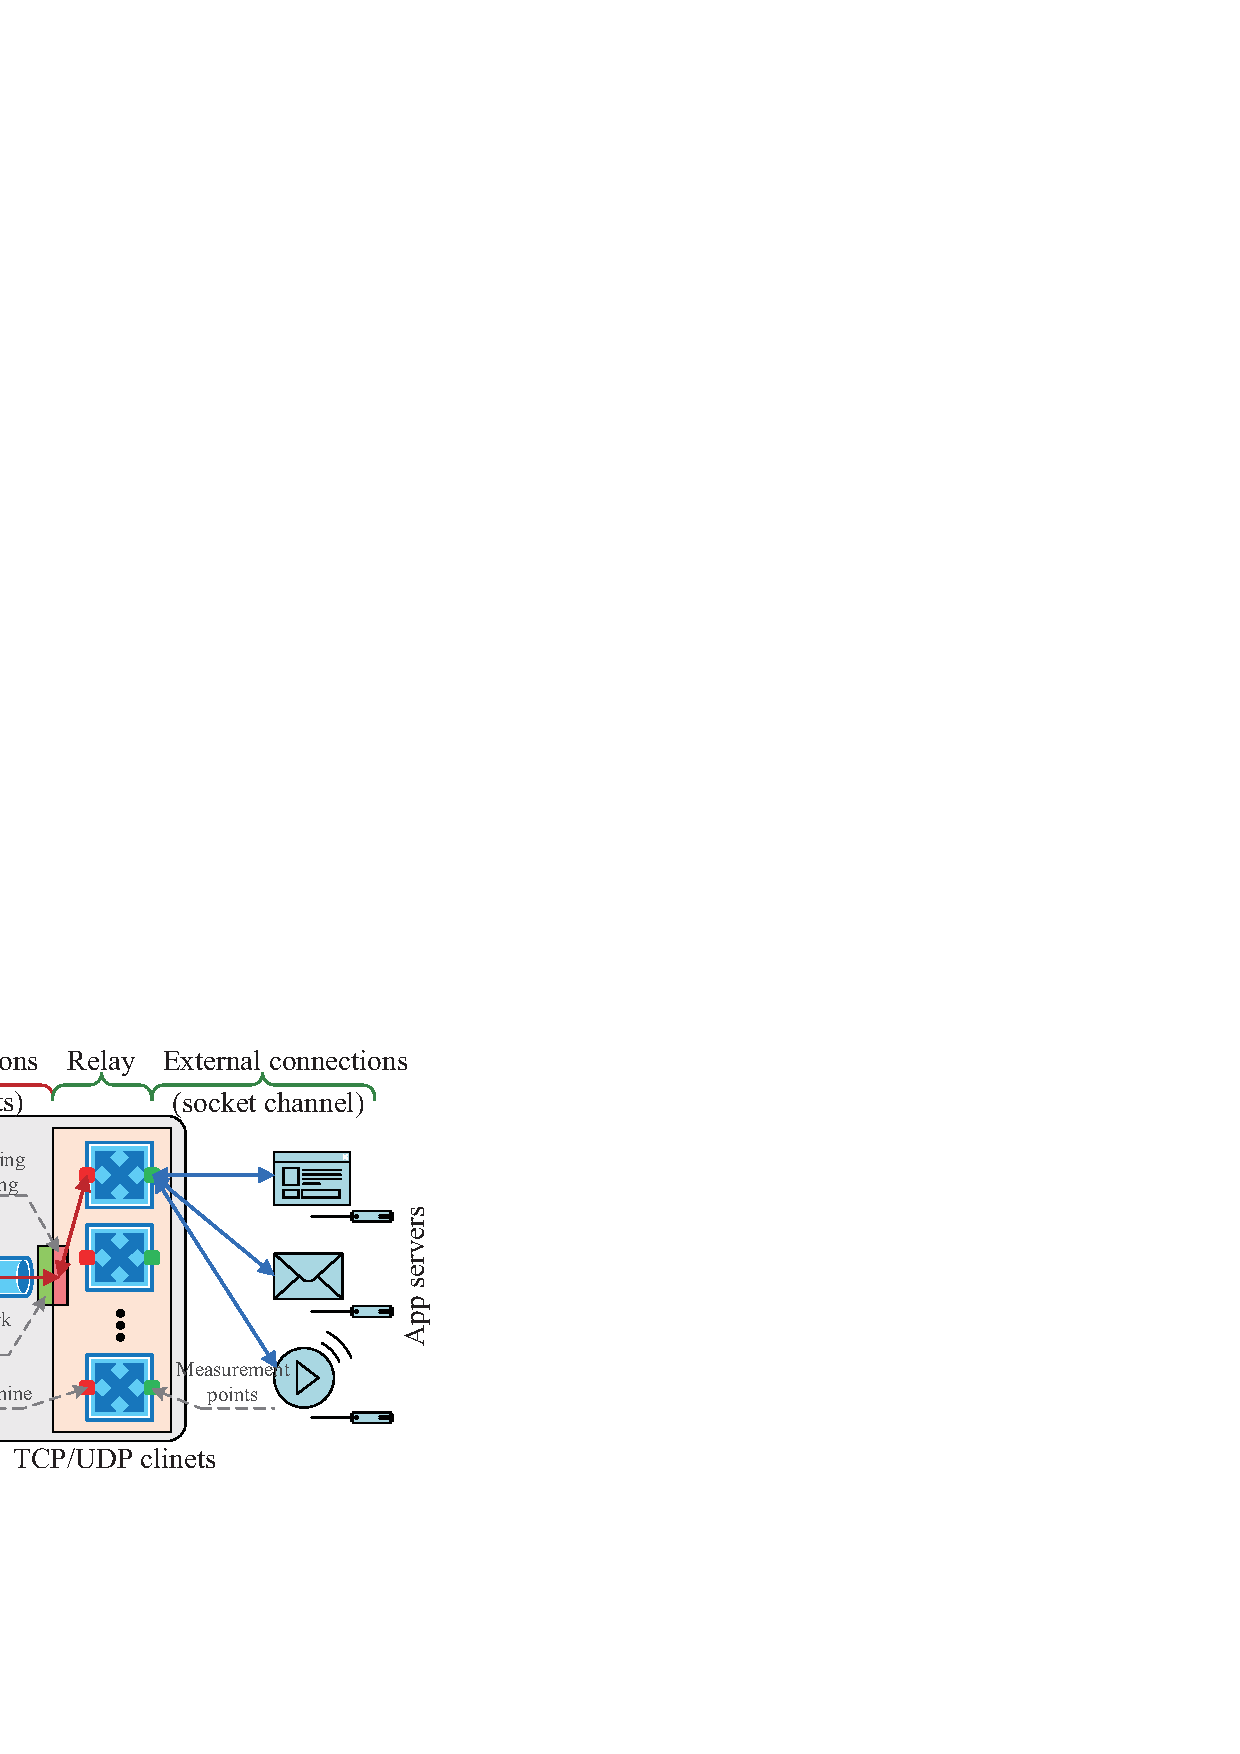
\includegraphics[width=\textwidth]{fig/mopeye.pdf}
        \end{column}
    \end{columns}
\end{frame}

% \begin{frame}
%     \frametitle{Data Features}
%     \begin{itemize}
%         \item User Information
%         \begin{itemize}
%             \item country, device model, android version, etc.
%             \item collects once per installation
%         \end{itemize}

%         \item Network Infromation
%         \begin{itemize}
%             \item type (WiFi or cellular), name (SSID or vendor name), geo-location etc.
%             \item collects each time on app enabled or network status changed
%         \end{itemize}

%         \item Measurement
%         \begin{itemize}
%             \item RTT, server IP and port, package name, the domain name etc.
%             \item measure each TCP connection or DNS query once.
%         \end{itemize}
%     \end{itemize}
% \end{frame}

% \begin{frame}
%     \frametitle{Basic Statistics}

%     \begin{columns}
%         \begin{column}{.35\textwidth}
%             \begin{itemize}
%                 \item Country Distribution: 11,200 users from 173 countries, mostly USA and Southeast Asia.
%             \end{itemize}
%         \end{column}

%         \begin{column}{.65\textwidth}
%             \includegraphics[width=\textwidth]{../fig/user_country.eps}
%         \end{column}
%     \end{columns}
% \end{frame}

% \begin{frame}
%     \frametitle{Basic Statistics}

%     \begin{columns}
%         \begin{column}{.35\textwidth}
%             \begin{itemize}
%                 \item Device Details: 1,615 different smartphone models from 226 manufacturers
%             \end{itemize}
%         \end{column}

%         \begin{column}{.65\textwidth}
%             \includegraphics[width=\textwidth]{../fig/phone_manufactory.eps}
%         \end{column}
%     \end{columns}
% \end{frame}

\begin{frame}
    \frametitle{Dataset}

    \begin{itemize}
        \setlength{\itemsep}{1.4em}
        % \item Country Distribution: 11,200 users from 173 countries, mostly USA and Southeast Asia.
        % \item Device Details: 1,615 different smartphone models from 226 manufacturers
        % \item Applications: 17,059 apps with 1,197 apps have $>$1k measurements
        % \item Network types: 65.42\% WiFi, 23.97\% LTE, 10.61\% other cellular networks.
        \item 20M records from 11k users in 173 countries.
        \item Interesting findings:
        \begin{itemize}
            \item only \textbf{5.94\%} of WiFi measurements were observed to have $>$300Mbps PHY rates.
            \item more than \textbf{one third} of the 653 ISPs have \textbf{no 4G} measurements observed, mainly in Africa and Asia.
        \end{itemize}
    \end{itemize}
\end{frame}
